\chapter{Results \textit{\&} Discussion}

\lettrine[
	nindent=0em, findent=0.5em, loversize=-0.12, lines=5
]{\initfamily{T}}{\bfseries\color{Blue}he proposed framework} is tested on the
\gls{uo} database, for predicting \ch{CO2} uptake in \glspl{mof}, the
gas\index{Gas} that mainly ``triggered'' the development of energy-based
descriptors\index{Energy-based descriptors}. In order to evaluate the
transferability of the approach, a different host-guest system is also examined.
We apply the suggested approach in the database created by
\textcite{Mercado_2018}, for predicting \ch{CH4} uptake in \glspl{cof}. In both
cases, the resulting \gls{ml} models are compared with conventional ones, built
upon geometric descriptors\index{Geometric descriptors}. In the rest of this
chapter, results from these comparisons are presented, followed by discussion
for improvements of the proposed framework. Before delving into the results, we
first take a look at RetNet\index{RetNet}, the 3D \gls{cnn} under the hood, that
takes as input a voxelized \gls{pes}\index{Voxelized PES} and outputs a
prediction for a gas adsorption\index{Gas adsorption} property, hereon gas
uptake.

\section{Visualizing RetNet}

Figure \ref{fig:retnet} illustrates the processing a voxelized PES undergoes, as
it is passing through RetNet. For the purpose of this visualization, we use the
model trained on the \glspl{mof} dataset with the largest training set size (see
Section \ref{sec:datasets}). Moreover, for the ease of visualization, only some
feature maps of RetNet are visualized. Please note, that each feature
map\index{Feature map} of a given layer, combines all the feature maps of the
precedent layer. The only exception are the pooling layers\index{Pooling layer},
which just downsample\index{Downsample} the feature maps from the previous
layers.

For example, each feature map of the \conv{2} layer takes into account all
the twelve feature maps of \conv{1} layer. In contrast, the feature maps of the
\pool{1} layer, are just downsampled versions of the corresponding feature maps
in \conv{2} layer. Although feature maps of \glspl{cnn} are not meant to be
interpreted by humans---especially the ones found deeper in the network---it is
worth noticing that early Conv layers\index{Conv layer} (i.e. \conv{1} and
\conv{2}) emphasize the texture of the structure. For instance, the third
feature map of \conv{1} layer delineates the skeleton of the framework.

Moving towards the output layer, the alternation of MaxPool and Conv layers
continues until the Flatten layer\index{Flatten layer}, which just flattens out
and concatenates\footnote{Given $m$ feature maps of size $n \times n \times n$,
a Flatten layer converts them into a vector of size $mn^3$.} all feature maps
from \conv{2} layer into a single vector of size \num{3240}. This vector is then
processed by a \gls{fcnn}---i.e. the stack of Dense\index{Dense layer} and
Output layers---to give the final prediction. Since the Output
layer\index{Output layer} is really nothing more than a linear
layer\index{Linear layer}, all that RetNet does is the following:

\begin{equation}
	\label{eq:retnet}
	\underbrace{\overbrace{\vcx}^\text{PES}}_\text{input}
	\quad \longrightarrow \quad
	\underbrace{
		\overbrace{\phi(\vcx;\vcth)}
		^\text{fingerprint}
	}_\text{feature extraction}
	\quad \longrightarrow \quad
	\underbrace{
		\overbrace{\vc{\beta}^\top\phi(\vcx;\vcth) + \beta_0}
		^\text{gas uptake}
	}_\text{output}
\end{equation}

\begin{figure}
	\centering
	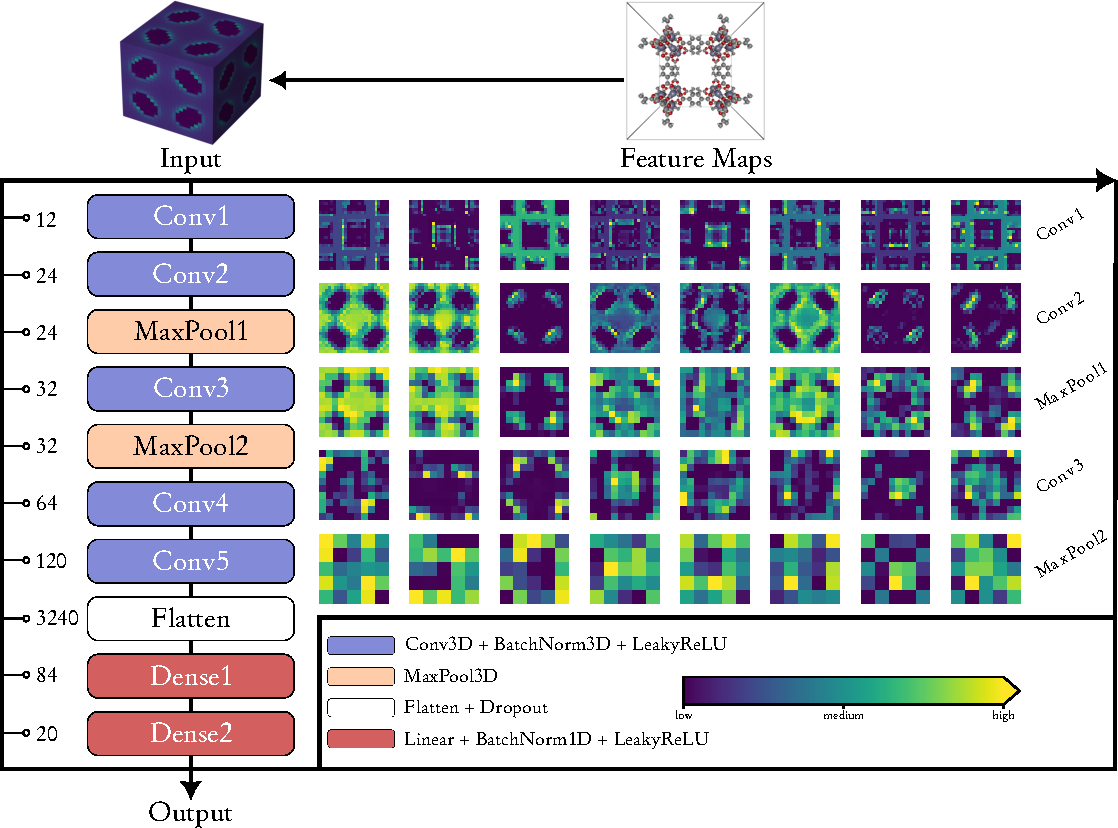
\includegraphics[width=\textwidth]{fig/forward_pass.pdf}
	\caption[RetNet architecture.]{Forward pass\index{Forward pass} of
	IRMOF-1\index{IRMOF-1} through RetNet\index{RetNet}. For the sake of
	visualization, only slices (feature maps\index{Feature map} are 3D matrices)
	of eight feature maps from the first five layers are visualized. For
	\conv{1} layer, the fifth slice is presented, while for the remaining
	layers, the first slice is presented. The IRMOF-1 structure was visualized
	with the iRASPA software \parencite{Dubbeldam2018}.}
	\label{fig:retnet}
\end{figure}

Equation \ref{eq:retnet} says that RetNet, \emph{starting from the PES,
extracts a fingerprint\index{Energetic fingerprint}---that is, a high level
representation\index{High level representation} of the \gls{pes}---and then
predicts the gas uptake by using a linear model on top of this fingerprint}. All
intermediate layers between Input\index{Input layer} and Output layer
participate in this feature extraction step, with the Dense\num{2} layer
determining the size of the fingerprint, which is a vector of size \num{20},
i.e. $\phi(\vcx) \in \mathbb{R}^{20}$ (see Figure \ref{fig:fingerprints}). The
fact that \emph{this fingerprint extraction\index{Fingerprint extraction} step
is learnable}---the parameters $\vcth$ of $\phi$ are learned during the training
phase\index{Training phase}---\emph{is what fundamentally distinguishes the
proposed approach from methods that use hand-crafted
fingerprints\index{Hand-crafted fingerprints}} (see Section
\ref{sec:literature}). \emph{In these methods the fingerprint or
extraction\index{Feature extraction} step is fixed}, and based on some
heuristic, such as energy histograms \parencite{bucior} or average interactions
\parencite{generic}. \emph{Hereon, feature extraction from the \gls{pes} is no
longer fixed, but is an essential part of the training phase}.

\begin{figure}
	\centering
	\begin{subfigure}[b]{0.49\textwidth}
		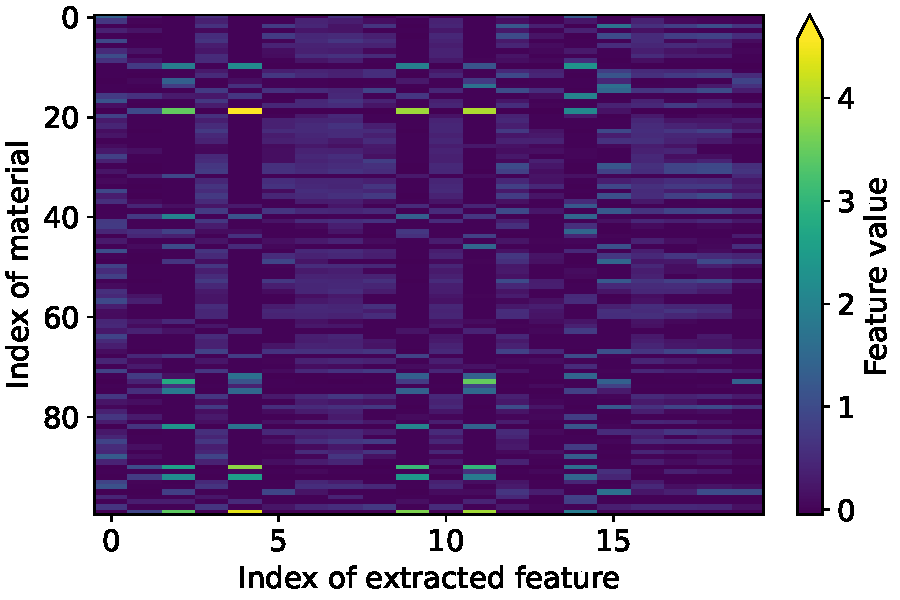
\includegraphics[width=\textwidth]{fig/extracted_features_mofs.pdf}
		\caption{Fingerprints extracted from the \glspl{mof} dataset.}
	\end{subfigure}
	\begin{subfigure}[b]{0.49\textwidth}
		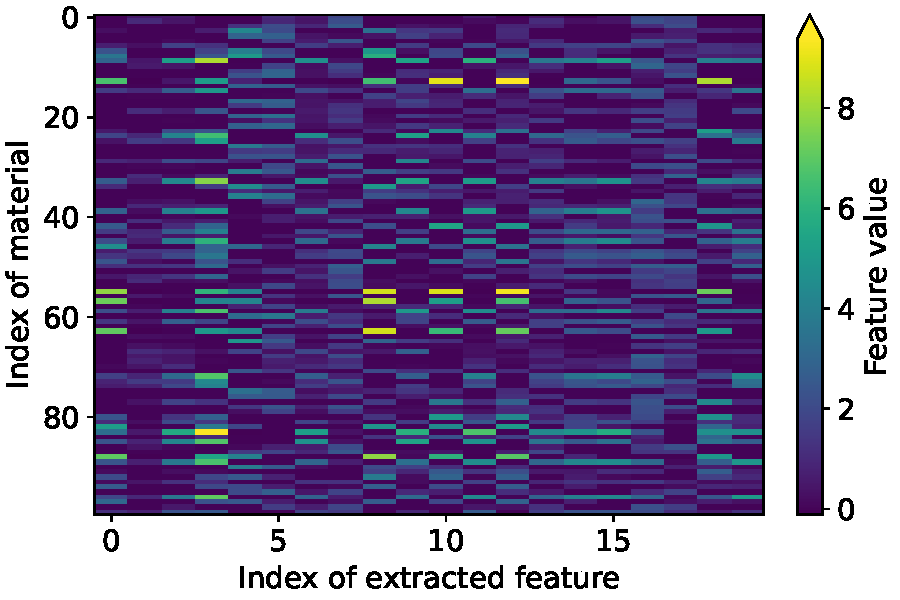
\includegraphics[width=\textwidth]{fig/extracted_features_cofs.pdf}
		\caption{Fingerprints extracted from the \glspl{cof} dataset.}
	\end{subfigure}
	\caption[Fingerprints extracted from RetNet.]{Output of the last LeakyReLU
	layer of RetNet trained on \glspl{mof} (left) and \glspl{cof} (right)
	datasets, with the corresponding maximum training set size. The fingerprints
	of the first \num{100} materials in the training set are depicted.}
	\label{fig:fingerprints}
\end{figure}

\section{Learning Curves}

The learning curves\index{Learning curve} of the conventional models---built
upon geometric descriptors---and the proposed ones--built upon energy
voxels---are shown in Figure \ref{fig:learning_curves_results}. As it can be
seen from Figure \ref{fig:learning_curves_mofs}, in the \gls{mof}-\ch{CO2} case,
the \gls{cnn} model achieves an $R^2$ score of \num{0.859}, outperforming the
conventional model, which shows an $R^2$ score of \num{0.690}. This amounts to
around \SI{25}{\percent} increase in accuracy, even with such a coarse
approximation of the \gls{pes}\footnote{In this work, all host-guest
interactions were modeled with the \gls{lj} potential (see Section
\ref{sec:voxelized_pes}), which neglects electrostatic interactions.}. Moreover,
from the same figure, one can notice that the proposed model reaches the peak
performance of the conventional one---that is, the performance when trained with
the maximum training set size---by requiring two orders of magnitude less
training data, around \num{300}.

Analogous results are observed when examining the \gls{cof}-\ch{CH4} case. Again
the \gls{cnn} model performs better, showing an $R^2$ score \num{0.969} compared
to \num{0.941} for the conventional one. Similar to the previous case, a
substantially smaller amount of training data are required---one order of
magnitude less training, around \num{6900}---for the \gls{cnn} model to match
the performance of the conventional model.

The fact that in both cases, the learning curves of the proposed models lie
above the corresponding ones of the conventional models, should be credited to
the following factors:
\begin{enumerate*}[label=\roman*).]
	\item The increased informativeness of the voxelized the voxelized
		\gls{pes}---in comparison to geometric descriptors.
	\item The ability of \glspl{cnn} to handle images and image-like
		data\index{Image-like data}, such as the voxelized \gls{pes}, which is
		essentially a single channel 3D image.
	\item The data augmentation\index{Data augmentation} technique, which was
		applied during the \gls{cnn} training (see Section
		\ref{subsec:data_augmentation}).
\end{enumerate*}

\begin{figure}
	\centering
	\begin{subfigure}[b]{0.49\textwidth}
		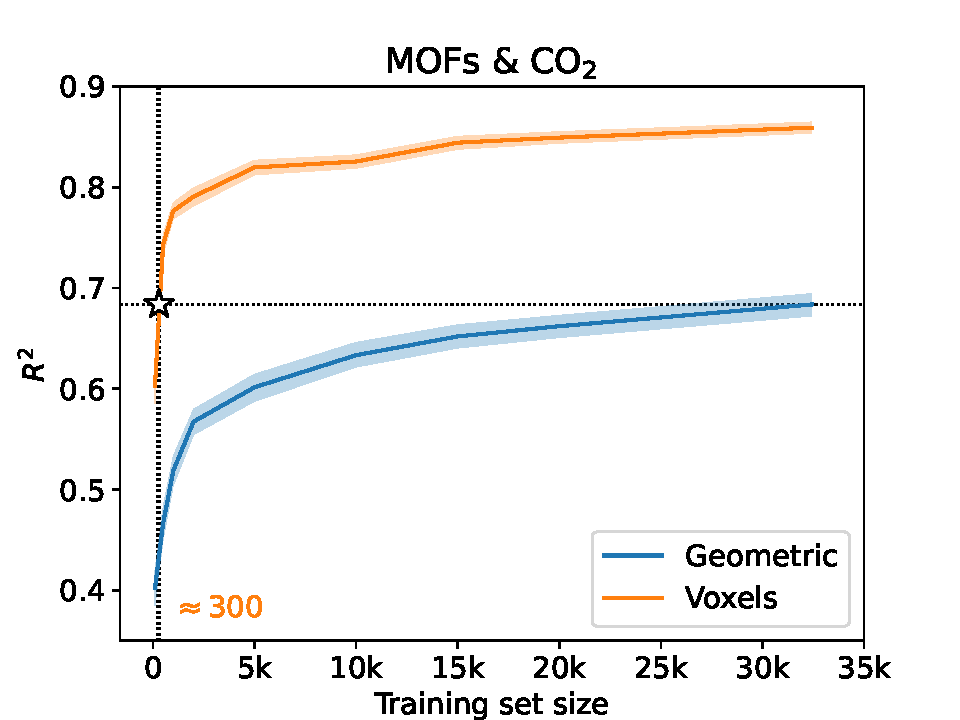
\includegraphics[width=\textwidth]{fig/learning_curves_mofs.pdf}
		\caption{Learning curves for \glspl{mof} \textit{\&} \ch{CO2}.}
		\label{fig:learning_curves_mofs}
	\end{subfigure}
	\begin{subfigure}[b]{0.49\textwidth}
		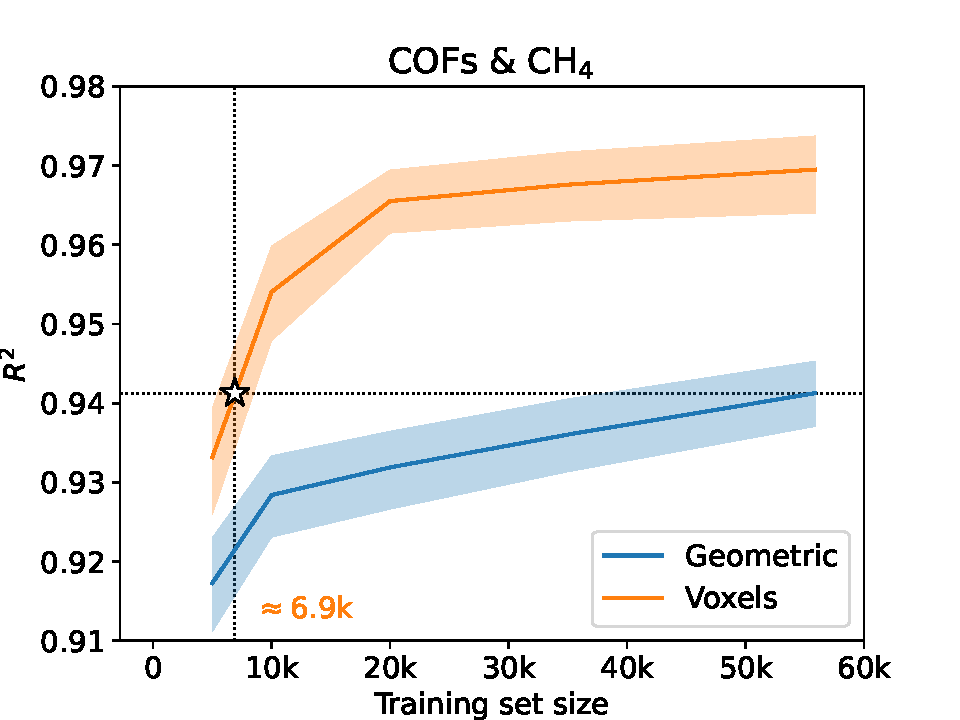
\includegraphics[width=\textwidth]{fig/learning_curves_cofs.pdf}
		\caption{Learning curves for \glspl{cof} \textit{\&} \ch{CH4}.}
		\label{fig:learning_curves_cofs}
	\end{subfigure}
	\caption[Learning curves.]{Performance ($R^2$ score) on test set as function
	of the training set size for conventional and \gls{cnn} models. Shaded areas
	correspond to the \SI{95}{\percent} \gls{ci}\index{Confidence interval}. The
	$x$-coordinate of the white star denotes the trainig set size where the
	\gls{cnn} model reaches the performance of the conventional one, the
	$y$-coordinate. ``Geometric'' stands for geometric descriptors, while
	``Voxels'' stands for energy voxels.}
	\label{fig:learning_curves_results}
\end{figure}

\section{Discussion}

It is worth mentioning the increase in performance, approximately
\SI{13}{\percent}, of the \gls{cnn} model in the \glspl{cof}-\ch{CH4} case
($R^2=0.969$) compared to the \glspl{mof}-\ch{CO2} case ($R^2=0.859$). In
contrast to \ch{CO2}, which exhibits strong electrostatic interactions with the
framework atoms, \ch{CH4} lacks dipole\index{Dipole moment} or quadrupole
moment\index{Quadrupole moment}. Given that the same resolution---i.e. the same
grid size---was used in both cases and that the \gls{lj} potential doesn't
account for electrostatic interactions, this performance gap should be
attributed to the absence of the latter in the voxelized \gls{pes}. \emph{In
other words, the extra ``contrast'' that such strong
interactions\index{Electrostatic interactions} add to the energy image of the
masterial, is missing from the voxelized \gls{pes}. As such, a straightforward
approach to improve the performance of the proposed approach, especially for
adsorbates like \ch{CO2}, \ch{H2} and \ch{H2S}, is to include this type of
interactions into the voxelized \gls{pes}}. Of course, there is no free lunch,
since these refinements require the assignment of partial charges\index{Partial
charge} to each framework atom, which is a computationally expensive task.
Luckily, \gls{ml}-based approaches have already been developed
\parencite{Bleiziffer2018, Raza2020, Kancharlapalli2021}, which can assign
partial charges rapidly and with high fidelity, enabling the efficient
construction of a more accurate voxelized \gls{pes}.

Improving the input, and as such, the performance of the suggested pipeline is a
major concern, but not the only one. \emph{What about the data
efficiency\index{Data efficiency} of the pipeline?} Imagine that we are asked to
predict \ch{CH4} uptake at various thermodynamic conditions\index{Thermodynamic
conditions}. A naive approach would be to collect training data\index{Training
data} and retrain from scratch the \gls{cnn} for every thermodynamic condition,
which is of course a laborious task. \emph{Can we do something smarter?} Well,
the fact that the proposed framework uses a \gls{dl} algorithm\index{Deep
learning algorithm} under the hood, opens the door for applying
\emph{\textbf{transfer learning} techniques}\index{Transfer learning}.  In a
nutshell, transfer learning\parencite{Zhuang2019, Ma2020, Kang2023} is based on
the following idea: \emph{a violist can learn to play piano faster than others,
since both the piano and the violin are musical instruments, and may share some
common knowledge.} Translating this to \glspl{nn}, a pre-trained \gls{nn} on an
original task---known as the \emph{source task}\index{Source task}---may require
less training data to perform well on a new task---known as the \emph{target
task}\index{Target task}---if there is some \emph{similarity between the tasks}.
Coming back to our ``imaginary'' scenario, all we have to do is to train the
\gls{cnn} once in a specific thermodynamic condition\footnote{Preferably, the
one where we have more labeled training data.} and then
fine-tune\index{Fine-tune} this pre-trained model\index{Pre-trained model} on
the other conditions.

Throughout this work we focused on gas adsorption, but of course this doesn't
mean we are not interested in predicting other properties of reticular
materials\index{Reticular materials}. \emph{What if we are asked to predict
properties such as band gap or bulk modulus?} In that case, quantities such as
\emph{electron density}\index{Electron density} are more informative over
host-guest interactions\index{Host-guest interactions} with regards to the
aforementioned properties. This entails that the \emph{voxelized electron
density}\index{Voxelized electron density} should substitute the voxelized
\gls{pes}, as input to the 3D \gls{cnn}. Nevertheless, \emph{\textbf{wouldn't be
great if all properties could be predicted from one and only one input?}} If our
aim is to predict \emph{different properties for the same structure, shouldn't
the structure itself be used as input?} Currently, the approaches to tackle this
challenge are based on \emph{text representations}\index{Text representations}
\parencite{Cao2023, Bucior2019} and \emph{crystal graphs}\index{Crystal graphs}
\parencite{Chen2019, Xie2018}. The main drawback of these approaches, is their
inability to represent exactly the structure, that is the \emph{exact
arrangement of the atoms in the 3D space}. \emph{\textbf{Point clouds}}
\parencite{Qi2016, Bello2020} are a natural way to solve this problem, since
they are just \emph{a set of coordinates\index{Coordinates} and associated
features}. In our context, the coordinates are the coordinates of the atoms, and
the associated features are the types of the atoms. It should be emphasized,
that \emph{a point cloud is not another mathematical
representation\index{Representation} of a material---in the sense of a
descriptor\index{Descriptor}---it is the material itself}\footnote{Same ideas
apply for molecules and in general, for any chemical system\index{Chemical
system}.}. Therefore, an answer to the original question is to \emph{couple
point clouds with a neural network that can handle such kind of input}. Such an
approach might has to overcome the current immaturity of \gls{dl} over point
clouds---especially regarding materials and molecules---but from a chemical
perspective, it is the only one that truly respects the 3D nature of chemistry
and of course, reticular chemistry.
